\documentclass{article}
\textwidth=6in
\hoffset=0in
\voffset=0in

\usepackage[a4paper, total={6in, 8in}]{geometry}
\usepackage{amsmath}
\usepackage{amssymb}
\usepackage{stmaryrd}
\usepackage{graphicx}
\usepackage{tikz}
\usetikzlibrary{automata, arrows}
\usepackage{pifont}
\usepackage{amssymb}
\usepackage{gensymb}
\usepackage{ngerman}
\usepackage[ampersand]{easylist}

% needs to be updated
\author{Max Springenberg, 177792}
\title{\
    GTI "Ubungsblatt 2\\
    Tutor: Marko Schmellenkamp\\
    ID: MS1\\
    "Ubung: Mi 16-18
    }
\setcounter{section}{2}
\date{}

% custom commands
% \Theta \Omega \omega
\newcommand{\tab}{\null\ \qquad}
\newcommand{\gap}{\null\ \\ \\}
\newcommand{\lA}{\leftarrow}
\newcommand{\rA}{\rightarrow}
\newcommand{\ue}{\infty}
\newcommand{\eps}{\epsilon}
\newcommand{\task}[1]{\textbf{#1} \\ \gap}
\newcommand{\cmark}{\ding{51}}
\newcommand{\xmark}{\ding{55}}
\newcommand{\degr}{\degree}

% content
\begin{document}
% title page
\maketitle
\newpage
% actual paper

\subsection\
\subsubsection{\
    Hannah arbeitet seit einiger Zeit an einem Webportal. Dieses soll nun so 
        erweitert werden, dass Lehrmaterialien in Form komprimierter oder 
        unkomprimierter Archivdateien hochgeladen werden k"onnen. Erlaubt sind
        TAR-Archive, eventuell mit GZIP komprimiert. G"ultig sind demnach die 
        Dateiendungen .tar, .tar.gz, .tgz. Der Einfachheit halber sei 
        vorausgesetzt, dass alle Dateinamen ausschlie"slich Kleinbuchstaben und
        Punkte beinhalten.\\
    Konstruieren Sie einen $\eps-NFA$ "uber dem Alphabet 
        $\Sigma= \{a, \ldots,z\}$ mit möglichst wenigen Zust"anden, der genau 
        die Dateinamen mit g"ultigen Dateiendungen akzeptiert.
    }
(i) F"ur alle W"orter der durch den Automaten entschiedenen Sprache $L$ gilt,
    dass sie vor der Dateiendung nicht das Zeichen `.' enthalten, aber beliebige 
    Teilw"orter aus $\{a, \ldots, z\}^* - \{\eps\}$.\\
Es wurde nichts zu einer Datei gesagt, die als einziges Teilwort vor der 
    Dateiendung das leere Wort enth"alt, aber auf Unix-System sind versteckte
    Dateien durch das Zeichen `.' am Anfang gekennzeichnet. So k"onnte `.tar'
    auch eine versteckte Datei mit Namen `tar' ohne Dateiendung sein.\\
(ii) Ferner muss auf mindestens eine Dateiendung aus der Menge 
    $\{.tar, .tar.gz, .tgz\}$ geendet werden. Es d"urfen keine anderen 
    Dateiendungen (wie z.B. .zip) als Teilstrings vorkommen, aber wir nehmen an,
    dass gueltige Dateiendungen aufeinander folgen d"urfen, da mehrfaches 
    vepacken m"oglich w"are.\\
\\
Konvention:\\
Hinsichtlich der "Ubersichtlichkeit werden Transitionen, wie auch in der 
    Vorlesung, die in den senkenden
    Zustand f"uhren weggelassen. Falls von einem Zustand aus also die Eingabe
    eines Zeichens nicht ber"ucksichtigt wird, ist das gleichbedeutend mit einer
    Transition in den senkenden Zustand.\\
\begin{tikzpicture}
    \node[initial, state](s)                    at (0,-4) {};
    \node[state](char)                          at (0,-2) {};
    \node[state](v_)                            at (0,0) {};
    \node[state](v_t)                           at (2,0) {};
    \node[state](v_ta)                          at (4,0) {};
    \node[accepting, state](v_tar)              at (6,0) {};
    \node[state](v_tar_)                        at (8,0) {};
    \node[state](v_tar_g)                       at (10,0) {};
    \node[accepting, state](v_tar_gz)           at (12,0) {};
    %\node[state](decl)                          at (6,-4) {};
    \path
        % verwerfen, bei leerem Wort
        (s)
            edge [->, left] node {a, ..., z} (char)
            %edge [->, above] node {.} (decl)
        (char)
            edge [->, loop left] node {a, ..., z} (char)
            edge [->, left] node {.} (v_)
        (v_)
            edge [->, above] node {t} (v_t)
            %edge [->, left] node {$\eps$} (decl)
        (v_t)
            edge [->, above] node {a} (v_ta)
            edge [->, bend right, above] node {$\eps$} (v_tar_)
        (v_ta)
            edge [->, above] node {r} (v_tar)
            %edge [->, left] node {$\eps$} (decl)
        (v_tar)
            edge [->, above] node {.} (v_tar_)
            edge [->, bend right, above] node {.} (v_)
        (v_tar_)
            edge [->, above] node {g} (v_tar_g)
            %edge [->, left] node {$\eps$} (decl)
        (v_tar_g)
            edge [->, above] node {z} (v_tar_gz)
            %edge [->, left] node {$\eps$} (decl)
        (v_tar_gz)
            edge [->, bend right, above] node {.} (v_)
        %(decl)
        %    edge [->, loop below] node {$\sigma \in \Sigma$} (decl)
        ;
\end{tikzpicture}\\
\subsubsection\
Die Aufgabe ist es einen DFA zu konstruieren, der W"orter, die nicht auf aa oder
    bb enden akzeptiert. Teilw"orter d"urfen jedoch auf aa, bb enden, wenn sie 
    nicht das letzte Teilwort sind.\\
Zudem soll der Automat nicht mehr als sieben Zust"ande besitzen.\\
Der Automat $A$ mit:\\
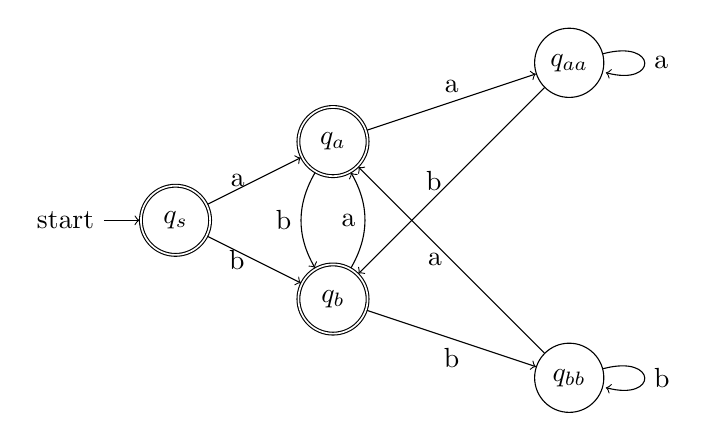
\begin{tikzpicture}
    \node[initial, accepting, state](s) at (0,0)  {$q_s$};
    \node[accepting, state](a)          at (2,1)  {$q_a$};
    \node[state](aa)                    at (5,2)  {$q_{aa}$};
    \node[accepting, state](b)          at (2,-1) {$q_b$};
    \node[state](bb)                    at (5,-2) {$q_{bb}$};
    \path
        (s)
            edge [->, left] node {a} (a)
            edge [->, left] node {b} (b)
        (a)
            edge [->, left, above] node {a} (aa)
            edge [->, bend right, left] node {b} (b)
        (aa)
            edge [->, loop right, right] node {a} (aa)
            edge [->, left] node {b} (b)
        (b)
            edge [->, bend right, left] node {a} (a)
            edge [->, below] node {b} (bb)
        (bb)
            edge [->, left] node {a} (a)
            edge [->, loop right, right] node {b} (bb)
        ;
\end{tikzpicture}\\
ist eine M"ogliche L"osung, da er nur f"unf Zust"ande besitzt und es gilt:\\
\\
Beim einlesens eines Zeichens $\sigma \in \Sigma$ nach einem zu $\sigma$
    unterschiedlichem Zeichen wird in den akzeptierenden Zustand $q_{\sigma}$ 
    gewechselt. Wird ein Zeichen direkt wieder eingelesen, so wird
    in den nicht akzeptierenden Zustand $q_{\sigma \sigma}$ gewechselt.\\
Ferner wird im Startzustand akzeptiert, da dass leere Wort in der Sprache
    enthalten ist.\\
In Konsequenz wird nur dann nicht akzeptiert, wenn ein Wort auf mindestens
    zweimal dem gleichem Zeichen endet.\\
\subsection\
\subsubsection\
\gap
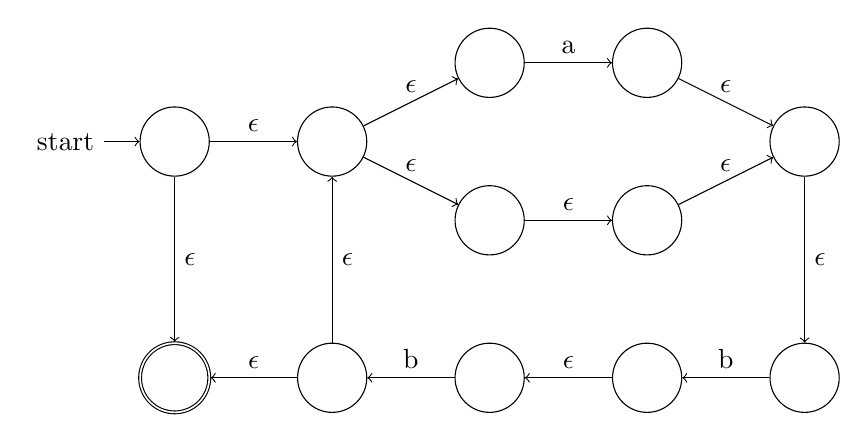
\begin{tikzpicture}
    \node[initial, state]   (1)  at (0,0) {};
    \node[state]            (2)  at (2,0) {};
    \node[state]            (3)  at (4,1) {};
    \node[state]            (4)  at (6,1) {};
    \node[state]            (5)  at (4,-1) {};
    \node[state]            (6)  at (6,-1) {};
    \node[state]            (7)  at (8,0) {};
    \node[state]            (8)  at (8,-3) {};
    \node[state]            (9)  at (6,-3) {};
    \node[state]            (10) at (4,-3) {};
    \node[state]            (11) at (2,-3) {};
    \node[accepting, state] (12) at (0,-3) {};
    \path
        (1) 
            edge [->, above] node {$\epsilon$} (2)
            edge [->, above, right] node {$\epsilon$} (12)
        (2) 
            edge [->, above] node {$\epsilon$} (3)
            edge [->, above] node {$\epsilon$} (5)
        (3) 
            edge [->, above] node {a} (4)
        (4) 
            edge [->, above] node {$\epsilon$} (7)
        (5) 
            edge [->, above] node {$\epsilon$} (6)
        (6) 
            edge [->, above] node {$\epsilon$} (7)
        (7) 
            edge [->, above, right] node {$\epsilon$} (8)
        (8) 
            edge [->, above] node {b} (9)
        (9) 
            edge [->, above] node {$\epsilon$} (10)
        (10)
            edge [->, above] node {b} (11)
        (11)
            edge [->, above] node {$\epsilon$} (12)
            edge [->, above, right] node {$\epsilon$} (2)
        ;
\end{tikzpicture}\\
\gap
Die Markierten Bereiche entsprechen den jeweiligen Teilw"ortern und entsprechen
    dem Baukastenprinzip aus der Vorlesung, damit ist dann auch der Automat 
    entsprechend dem Baukastenprinzip der Vorlesung aufgebaut.\\
\subsubsection\
Die $\eps$-closures aller Knoten erbegen sich zu:\\$
    \eps\text{-clousre}(1) = \{3,2\} 
        \text{, mit } 1 \rightarrow^\eps 3 \rightarrow^\eps 2\\
    \eps\text{-clousre}(2) = \emptyset 
        \text{, mit } \nexists q \in Q : 2 \rightarrow^\eps q\\
    \eps\text{-clousre}(3) = \{2\}
        \text{, mit } 3 \rightarrow^\eps 2\\
    \eps\text{-clousre}(4) = \emptyset
        \text{, mit } \nexists q \in Q : 4 \rightarrow^\eps q\\
    $\\
Der folgende Automat $A$:\\
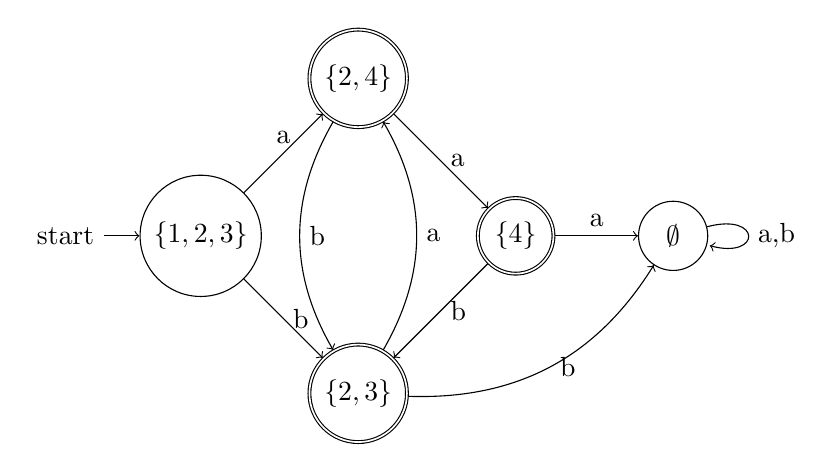
\begin{tikzpicture}
    \node[initial, state](123)  at (0,0)  {$\{1,2,3\}$};
    \node[accepting, state](24)  at (2,2)  {$\{2,4\}$};
    \node[accepting, state](4)  at (4,0)  {$\{4\}$};
    \node[accepting, state](23) at (2,-2) {$\{2,3\}$};
    \node[state](empty)         at (6,0) {$\emptyset$};
    \path
        (123)
            edge [->, above] node {a} (24)
            edge [->, right] node {b} (23)
        (4)
            edge [->, above] node {a} (empty)
            edge [->, right] node {b} (23)
        (23)
            edge [->, bend right, right] node {a} (24)
            edge [->, bend right, right] node {b} (empty)
        (24)
            edge [->, right] node {a} (4)
            edge [->, bend right, right] node {b} (23)
        (empty)
            edge [->, loop right] node {a,b} (empty)
        ;
\end{tikzpicture}\\
ist eine m"ogliche L"osung.\\
\\
Der Startzustand umfasst die Menge $\{1,2,3\}$, da dies der $\eps$-closure vom 
    Startzustand 1 entspricht.\\
Jeder akzeptierender Zustand ist genau dann ein solcher, wenn er in seiner Menge
    mindestens einen akzeptierenden Zustand (2 oder 4) enth"alt.\\
Die Transitionen von einem Zustand $q$ bei Eingabe des Zeichens $\sigma$ ergeben 
    sich "uber die Konkatenation von $P_1, \ldots, P_n$ mit 
    $q_k \rightarrow^{\sigma} P_k, 1 \leq k \leq n$ f"ur alle 
    $q_1,\ldots,q_n \in q$, wobei $P_k$ die jeweilige Menge von Zust"anden die 
    durch Eingabe von $\sigma$ erreicht werden k"onnen, bzw. closure ist.\\
Ferner gilt, dass dabei auch alle Zust"ande in der jeweiligen Menge eines 
    Zustands mit den jeweiligen $\eps$-closures konkateniert wurden und damit 
    auch alle $\eps$-closures ber"ucksichtigt wurden.\\
\subsubsection\
Uns interessieren nur die Ausdr"ucke $\alpha_{2,2}^{2}, \alpha_{1,2}^{2}$, da 2
    der einzige Akzeptierende Zustand ist.\\
wir alhalten $\alpha_{acc} = \alpha_{2,2}^{2} + \alpha_{1,2}^{2}$ mit:\\
\\$
    \alpha_{1,1}^{0} = a + c\\
    \alpha_{2,2}^{0} = a + b\\
    \alpha_{1,2}^{0} = b\\
    \alpha_{2,1}^{0} = c\\
    \gap
    \alpha_{1,1}^{1} 
        = \alpha_{1,1}^{0}
            + \alpha_{1,1}^{0}(\alpha_{1,1}^{0})^* \alpha_{1,1}^{0}
        \equiv (a+c) + (a+c)(a+c)^*(a+c) 
        \equiv (a+c)(a+c)^*\\
    \alpha_{2,2}^{1}
        = \alpha_{2,2}^{0} 
            + \alpha_{2,1}^{0}(\alpha_{1,1}^{0})^* \alpha_{1,2}^{0}
        \equiv (a+b) + c(a+c)^*b\\
    \alpha_{1,2}^{1}
        = \alpha_{1,2}^{0} 
            + \alpha_{1,1}^{0}(\alpha_{1,1}^{0})^* \alpha_{1,2}^{0}
        \equiv b + (a+c) (a+c)^* b
        \equiv (a+c)^* b\\
    \alpha_{2,1}^{1}
        = \alpha_{2,1}^{0} 
            + \alpha_{2,1}^{0}(\alpha_{1,1}^{0})^* \alpha_{1,1}^{0}
        \equiv c + c (a+c)^* (a+c)
        \equiv c (a+c)^*\\
    \gap
    \alpha_{1,2}^{2}
        = \alpha_{1,2}^{1}
            + \alpha_{1,2}^{1}(\alpha_{2,2}^{1})^* \alpha_{2,2}^{1}\\
    \equiv ((a+c)^*b) 
        + ((a+c)^*b) ((a+b) + c(a+c)^*b)^* ((a+b) + c(a+c)^*b)\\
    \equiv (a+c)^*b ((a+b) + c(a+c)^*b)^*\\
    \\
    \alpha_{2,2}^{2}
        = \alpha_{2,2}^{1}
            + \alpha_{2,2}^{1}(\alpha_{2,2}^{1})^* \alpha_{2,2}^{1}\\
    \equiv ((a+b) + c(a+c)^*b)
        + ((a+b) + c(a+c)^*b) ((a+b) + c(a+c)^*b)^* ((a+b) + c(a+c)^*b)\\
    \equiv (a+b) + c(a+c)^*b ((a+b) + c(a+c)^*b)^*\\
    $\\
zu:\\
$
    \alpha_{acc} 
        = (a+c)^*b ((a+b) + c(a+c)^*b)^*
            + (a+b) + c(a+c)^*b ((a+b) + c(a+c)^*b)^*\\
    \equiv (a+b) + c^* (a+c)^*b ((a+b) + c(a+c)^*b)^*
    $\\
\subsection\
Die Sprachen:\\
$
    W_0 = \{w \in \{a,b\}^* |\ |w| \text{ gerade}\}\\
    W_1 = \{w \in \{a,b\}^* |\ |w| \text{ ungerade}\}\\
    W_2 = \{w \in \Sigma^* | \#_c(w) > 0\}\\
    $\\
Sind korrekt, da:\\
Eingaben aus $\{a,b\}^*$ die Zust"ande 0 und 1 abwechselnd durchlaufen. Dabei 
    wird im Zustand 0 gestartet und die erste Transition nach Eingabe $\sigma
    \in \{a,b\}$ f"uhrt in 1. In Konsequenz sind W"orter aus 0 und 1 "uber 
    $\{a,b\}$ und alle W"orter in 1 ungerade und in 0 gerade.\\
Nach einlesem des erstem c wird in den Zustand 2 gewchselt und dort f"ur alle
    Eingaben geblieben. Damit enthalten alle W"orter in 2 mindestens ein c, sind
    sonst aber beliebig\\
\gap
Ferner gilt $L(A) = (W_0 - W_1) - W_2$\\
Offensichtlich gilt $(W_0 - W_1) = W_0$ und damit $L(A) = W_0 - W_2$.
    $L(A) = W_0 - W_2$ ergibt sich zu:\\
\[
    L(A) = \{w \in \{a,b\}^* |\ |w| \text{ gerade}\}
        - \{w \in \Sigma^* | \#_c(w) > 0\}
    = \{w \in \Sigma^* |\ |w| \text{ gerade} \land \#_c(w) = 0\}
    = L\\
    \]
\end{document}
